\chapter{INTERNSHIP ACTIVITIES}

The internship was carried out over a period of six weeks, providing a structured and continuous learning journey. The activities progressed from foundational concepts in Artificial Intelligence and Machine Learning to practical applications in Data Science, ultimately leading to advanced Computer Vision projects. This chapter presents the chronological sequence of learning, highlighting the technologies explored and the practical tasks completed during each week.

\section{Week 1: Introduction to AI and Mini Projects}

The first week focused on establishing a strong foundation in the fundamentals of Artificial Intelligence (AI) and Machine Learning (ML). The internship commenced with an orientation session where the mentors outlined the internship objectives, the modern technology stack to be covered, and the practical projects scheduled for the six-week training period.

Theoretical sessions covered essential concepts, including:
\begin{itemize}[leftmargin=1.5cm]
    \item Artificial Intelligence, Machine Learning, and Deep Learning
    \item Large Language Models (LLMs)
    \item Application Programming Interfaces (APIs)
    \item Model Context Protocol (MCP)
    \item The AI Development Workflow
\end{itemize}

\subsection{AI Translator Project}

The first practical activity was the development of an AI Translator application. 

\textbf{Introduction:} The AI Translator serves as a fundamental example of how AI models process human language. It converts text from a source language into a target language using automated translation models.

\textbf{Objective:} To understand text-to-text conversion mechanisms and familiarize with the architecture of AI-based applications.

\textbf{Technologies Used:} Python, Flask, HTML, CSS, JavaScript, and translation APIs.

\textbf{Methodology \& Implementation:} The application architecture followed a standard web development pattern. The frontend, designed using HTML and CSS, collected user input and the desired target language. The Python and Flask backend processed this input, transmitted it to the translation API, and returned the translated text. This mini-project demonstrated how frontend and backend components interact seamlessly in AI applications.

\textbf{Learning Outcome:} The project provided practical exposure to handling text data and illustrated how mini-projects serve as building blocks for understanding complete AI workflows.

\begin{figure}[H]
\centering
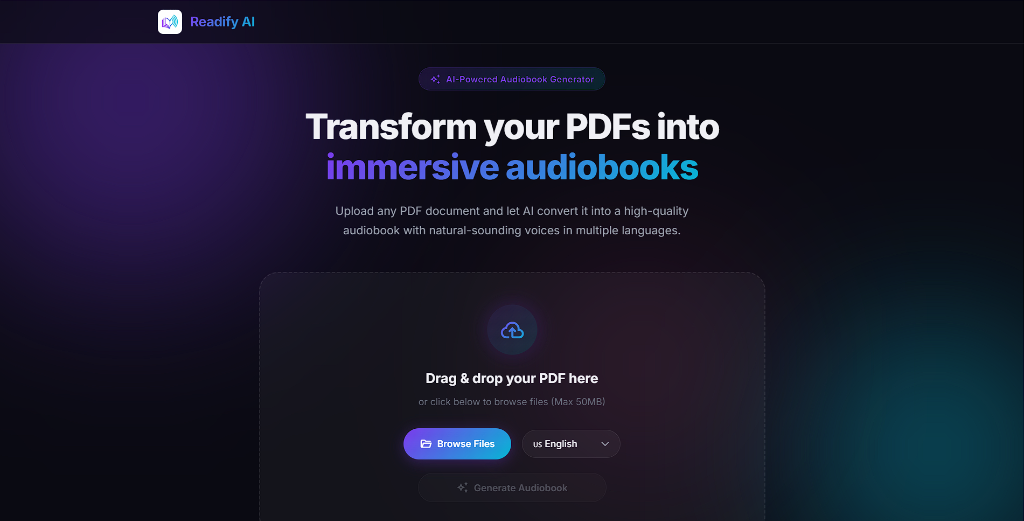
\includegraphics[width=0.8\textwidth]{images/readify_ai.png}
\caption{Readify AI - PDF to Audiobook Interface}
\label{fig:readify_ai}
\end{figure}

\subsection{Text-to-Speech Project}

The second learning activity involved developing a web-based Text-to-Speech (TTS) application.

\textbf{Introduction:} TTS systems convert written text into spoken audio output. This project introduced the integration of Google Text-to-Speech (gTTS) within a web framework.

\textbf{Objective:} To understand audio generation from text and implement voice control features in a web application.

\textbf{Technologies Used:} \cite{python} Python, Flask, HTML, CSS, JavaScript, and gTTS.

\textbf{Methodology \& Implementation:} The application was designed to accept text input, allow language selection, and control speech speed. The Flask backend utilized the gTTS library to process the text and generate an audio file. The generated audio files were stored locally and served back to the frontend for playback. The folder structure was carefully organized into Python files, templates, and static resources to maintain clean architecture.

\textbf{Learning Outcome:} The project clarified the role of gTTS in audio generation and demonstrated how Python handles file generation and serving within a Flask application.

\subsection{Weather API Project}

Students were introduced to the concepts of REST APIs, HTTP Requests, and JSON data parsing.

\textbf{Introduction:} APIs are the backbone of modern AI systems, allowing disparate software systems to communicate.

\textbf{Objective:} To perform data collection by communicating with an external REST API.

\textbf{Technologies Used:} Python, Pandas, Requests Library, BeautifulSoup, OpenWeather API.

\textbf{Methodology \& Implementation:} The project involved sending HTTP requests to the OpenWeather API. The resulting JSON response was parsed to extract relevant weather parameters. The extracted data was formatted and displayed to the user. Python's Requests library was utilized for API communication, while Pandas was introduced for structuring the collected data.

\textbf{Learning Outcome:} The activity provided crucial experience in real-world API integration, demonstrating how data is fetched, parsed, and utilized dynamically.

\section{Week 2: Data Analysis and Visualization}

The second week introduced Data Science concepts, focusing heavily on data preprocessing, which is a critical stage before any model training. The quality of a machine learning model is directly proportional to the quality of the data it is trained on.

Theoretical topics covered included data cleaning, missing value handling, feature engineering, and statistical analysis. Python libraries such as \cite{numpy} NumPy, SciPy, \cite{pandas} Pandas, and \cite{matplotlib} Matplotlib were extensively utilized.

\subsection{Cars Dataset Analysis}

A complete Exploratory Data Analysis (EDA) was performed on a dataset containing automobile specifications.

\textbf{Objective:} To understand the structure of raw data and perform necessary cleaning operations.

\textbf{Methodology \& Implementation:} 
The dataset was loaded using Pandas. Initial data inspection revealed missing values and unnecessary columns, which were systematically removed or imputed. Columns were renamed for consistency, and descriptive statistics were generated. 

To understand the dataset visually, multiple charts were plotted using Matplotlib, including histograms for distribution analysis, box plots for outlier detection, scatter plots for variable relationships, and correlation heatmaps and pair plots for multidimensional analysis. The AutoViz library was also explored to automate the visualization process.

\textbf{Learning Outcome:} The project emphasized the importance of visualization in understanding datasets, revealing patterns and brand distributions that were not apparent in raw tabular data.

\begin{figure}[H]
\centering
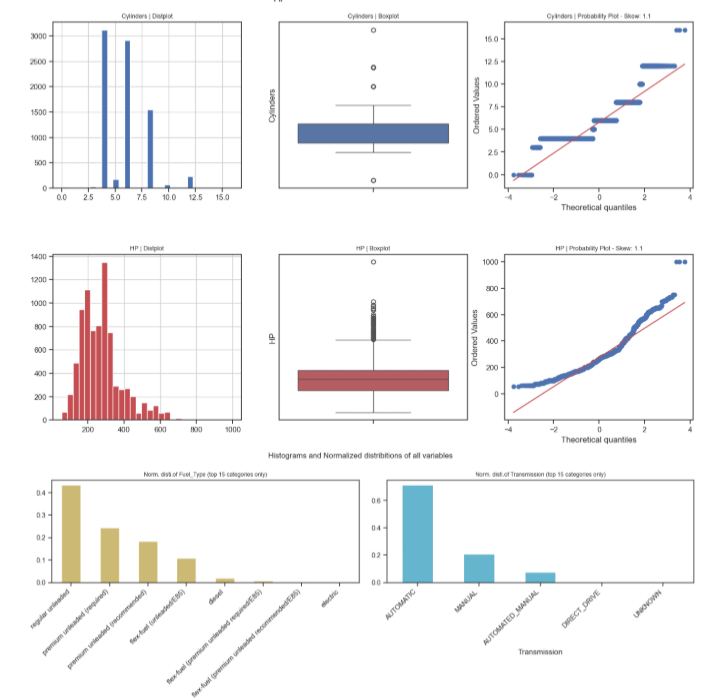
\includegraphics[width=0.7\textwidth]{images/autoviz_cars.png}
\caption{Exploratory Data Analysis on Cars Dataset}
\label{fig:cars_eda}
\end{figure}

\subsection{Placement Dataset Analysis}

A placement dataset containing student academic details was analyzed to identify factors influencing employability.

\textbf{Dataset Features:} SSC Percentage, HSC Percentage, Degree Percentage, MBA Percentage, Employability Test score, Specialization, Work Experience, Placement Status, and Salary.

\textbf{Methodology \& Implementation:} The data was cleaned and visualized to perform correlation analysis. Placement trends were analyzed in relation to academic percentages and work experience. Feature relationships were explored to determine which academic metrics most strongly correlated with higher salary packages.

\textbf{Learning Outcome:} The analysis provided practical insights into how feature engineering and statistical analysis can uncover meaningful trends in educational data.

\subsection{Introduction to Machine Learning}

The latter part of the week focused on formalizing Machine Learning concepts. 

The differences between Supervised Learning, Unsupervised Learning, and Reinforcement Learning were discussed. Within supervised learning, the concepts of Regression and Classification were explored in depth. 

The theoretical foundations of various algorithms were covered, including:
\begin{itemize}[leftmargin=1.5cm]
    \item Linear and Logistic Regression
    \item Decision Tree and Random Forest
    \item K-Nearest Neighbors (KNN)
    \item Naive Bayes
    \item Support Vector Machine (SVM)
    \item Multi-Layer Perceptron (MLP)
    \item XGBoost and Voting Classifier Ensembles
\end{itemize}

Model evaluation techniques were also introduced, explaining metrics such as Accuracy, Precision, Recall, F1 Score, Confusion Matrix, Mean Squared Error (MSE), Mean Absolute Error (MAE), and R² Score.

\section{Week 3: Machine Learning Projects}

Week 3 involved the practical implementation of the machine learning algorithms discussed previously.

\subsection{Student Performance Prediction}

\textbf{Objective:} To predict a student's final grade (G3) based on demographic, social, and academic features.

\textbf{Methodology \& Implementation:} 
Data cleaning and One-Hot Encoding were performed to convert categorical variables into numerical formats. Extensive EDA and correlation analysis were conducted to select the most relevant features. The dataset was split into training and testing sets. Multiple models, including Random Forest, Decision Tree, and KNN, were trained. 

\textbf{Results:} The models were compared based on their predictive performance. Feature importance analysis revealed that previous academic scores were the strongest predictors of the final grade.

\textbf{Learning Outcome:} The project provided a complete walkthrough of the standard ML pipeline, from data ingestion to model evaluation.

\subsection{Titanic Survival Prediction}

\textbf{Objective:} To predict passenger survival on the Titanic based on passenger attributes.

\textbf{Methodology \& Implementation:}
Handling missing values and feature engineering were the core focus. New features such as `FamilySize` and `IsAlone` were created, and titles were extracted from passenger names. Numerical features were standardized using Standard Scaling, and SelectKBest was used for feature selection.

A wide array of classification algorithms was trained: Logistic Regression, Random Forest, Decision Tree, KNN, Naive Bayes, SVM, MLP, XGBoost, and a Voting Classifier.

\textbf{Results:} The models were evaluated using accuracy scores and confusion matrices. The best performing model was utilized to generate a CSV submission file containing the predictions.

\textbf{Learning Outcome:} The project highlighted how thoughtful feature engineering significantly improves model performance, often more so than algorithmic tuning.

\subsection{AutoViz and Automated EDA}

The use of AutoViz for automated exploratory data analysis was discussed. While AutoViz provides rapid automatic visualization and highlights correlations quickly, it was noted that compatibility issues with specific Matplotlib and Seaborn versions can occur. The debugging process reinforced the importance of understanding the underlying libraries even when utilizing automated tools.

The foundational data science and machine learning skills acquired during the first three weeks smoothly transitioned into the advanced computer vision projects undertaken in the subsequent weeks.
